\documentclass[letterpaper]{article} % DO NOT CHANGE THIS
\usepackage[submission]{aaai2027}  % DO NOT CHANGE THIS
\usepackage[hyphens]{url}  % DO NOT CHANGE THIS
\usepackage{graphicx} % DO NOT CHANGE THIS
\urlstyle{rm} % DO NOT CHANGE THIS
\def\UrlFont{\rm}  % DO NOT CHANGE THIS
\usepackage{natbib}  % DO NOT CHANGE THIS AND DO NOT ADD ANY OPTIONS TO IT
\usepackage{caption} % DO NOT CHANGE THIS AND DO NOT ADD ANY OPTIONS TO IT
\frenchspacing  % DO NOT CHANGE THIS
\usepackage{algorithm}
\usepackage{algorithmic}
\usepackage{newfloat}
\usepackage{listings}
\DeclareCaptionStyle{ruled}{labelfont=normalfont,labelsep=colon,strut=off} % DO NOT CHANGE THIS
\lstset{%
	basicstyle={\footnotesize\ttfamily},
	numbers=left,numberstyle=\footnotesize,xleftmargin=2em,
	aboveskip=0pt,belowskip=0pt,%
	showstringspaces=false,tabsize=2,breaklines=true}
\floatstyle{ruled}
\newfloat{listing}{tb}{lst}{}
\floatname{listing}{Listing}
\usepackage{booktabs}
\usepackage{amsmath}
\usepackage{amssymb}
\pdfinfo{
/TemplateVersion (2027.1)
}
\setcounter{secnumdepth}{0}

\title{Physics-Constrained Conditional Flows for\\Liquefaction Onset Forecasting}
\author{Anonymous Submission}
\affiliations{Paper under double-blind review}

\begin{document}
\maketitle

\begin{abstract}
Soil liquefaction is a high-consequence failure mode, yet each cyclic laboratory test that characterizes
it can take days to weeks and specialized equipment to run, so the data are intrinsically scarce.
Engineering practice compresses a cyclic process into a single triggering boundary, rather than
forecasting the pore-pressure response and the time to onset from a partial early observation.
We cast laboratory liquefaction assessment as \emph{prefix-conditioned probabilistic event-time
forecasting}: from static soil/loading descriptors and an early excess pore-pressure (PPR) prefix,
predict the PPR continuation, liquefaction risk, and the (possibly right-censored) cycle count to onset.
We introduce \textbf{DPI-Flow}, a physics-structured architecture that amortizes inference of physically
constrained parameters through a \emph{conditional coupling (RealNVP) flow} and rolls them through a
\emph{differentiable analytical CRR/damage/PPR layer}, guaranteeing feasible monotone accumulation;
a censoring-aware objective uses exact event times and right-censored non-events, and a Monte-Carlo
predictive propagates uncertainty through the flow. The archive contains \textbf{1{,}093 raw tests across
20 sites}; the strict landmark benchmark contains \textbf{790 tests across 14 sites} after excluding both
events and censoring before the landmark. We evaluate all models with nested object-held-out cross-validation,
object-cluster uncertainty intervals, post-prefix metrics, and explicit physical-regime stratification.
\end{abstract}

\section{Introduction}
Soil liquefaction---the loss of effective stress in saturated granular soil under cyclic loading---is a
high-consequence dynamic failure that drives large economic losses and threatens lives and
infrastructure. Engineering practice evaluates it through the cyclic stress ratio / cyclic resistance
ratio (CSR/CRR) ``simplified procedure'' and its probabilistic successors
\citep{seedidriss71,youd01,boulanger16}. These procedures are well established, but they compress a
cyclic process into a triggering boundary or probability, rather than forecasting the full excess
pore-pressure trajectory $\mathrm{PPR}(N)$ and the event time under partial early observations.

Machine-learning models for liquefaction have grown rapidly, yet they have been criticized for weak
comparison to state-of-practice, insufficient validation, limited reproducibility, and a tendency to
treat the problem as static classification \citep{maurer23,jas23,sanger25}. This is precisely the
\emph{small, expensive, site-specific data} regime that data-centric geotechnics identifies as needing
strong inductive bias and honest, site-aware evaluation \citep{phoon22,baghbani22}. The same dynamic
instability of saturated sands is studied with constitutive and laboratory models in the geotechnical
literature \citep{termart25,termart23,sidorov24}, while recent data-driven work increasingly targets
transfer across sites and probabilistic assessment \citep{guotransfer25,demir24}. Crucially, each
datum here is costly ground truth obtained from a multi-day physical experiment, so the scientific
question is not how to fit large data but how to extract maximal signal per experiment.

We formulate laboratory liquefaction assessment as \emph{prefix-conditioned probabilistic event-time
forecasting}: given static soil/loading descriptors and an early PPR prefix, predict the continuation of
$\mathrm{PPR}(N)$, the probability of liquefaction, and the censored time-to-event $N_{\mathrm{liq}}$.
This connects scientific machine learning, latent-variable inference, neural differential equations,
normalizing flows, uncertainty calibration, and survival/event-time modeling
\citep{karniadakis21,chen18,latentnode22,rezende15,guo17,romano19,cuqds25,davis06,abdar21,cox72}.

We introduce \textbf{DPI-Flow}, a physics-structured probabilistic model that amortizes inference of
physically constrained latent parameters $\theta$, refines them through prefix calibration, and
integrates a differentiable analytical CRR/damage/PPR layer; uncertainty is propagated through the flow
by Monte-Carlo sampling at inference. Our contributions are: (i) a \textbf{prefix-conditioned
onset-forecasting formulation} for cyclic liquefaction tests; (ii) a \textbf{conditional parameter flow
plus differentiable analytical layer} that guarantees feasible monotone accumulation while producing
risk, $N_{\mathrm{liq}}$ and a CRR curve from one latent state; (iii) a \textbf{censoring-aware
objective} that separates exact events, right-censored event times, and by-horizon risk observability;
(iv) an \textbf{object-held-out landmark benchmark} on 790 tests from a 1{,}093-test archive with strong tabular, sequence and
physics-informed baselines and object-cluster confidence intervals; and (v) a \textbf{transparent
uncertainty/physics evaluation}. Under honest evaluation, DPI-Flow is not best on every individual metric;
it is the best \emph{physically admissible} Pareto balance---a more defensible and, we argue, more useful
result for engineering practice.

\section{Problem Setup}
\paragraph{Task.} A cyclic test is observed on a cycle grid $N_1<\dots<N_T$. For specimen $i$ we have
static descriptors $s_i\in\mathbb{R}^{d_s}$ (soil physical/mechanical properties and loading parameters),
a cyclic-stress history $c_i\in\mathbb{R}^{T}$ with $c_{it}=\mathrm{CSR}_i(N_t)$, and an early
\emph{prefix} of the measured excess pore-pressure ratio $r_{i,1:L}$ with $L$ the prefix length. The onset
is the first threshold crossing $N^\star_i=\min\{N_t: r_i(N_t)\ge\tau\}$ with $\tau=0.95$, the label is
$y_i=\mathbf{1}[N^\star_i\le N_T]$, and $N_{\mathrm{liq},i}=N^\star_i$ (or right-censored at $N_T$). The
targets are the continuation $r_i(N_t)$ for $N_t>N_L$, the risk $y_i$, and the censored event time
$N_{\mathrm{liq},i}$.

\paragraph{Strictly pre-onset prefix.} The observed prefix is truncated \emph{strictly before onset}: no
prefix step is at or beyond the onset cycle. Without this, fast tests leak the event into the input and
inflate onset metrics; enforcing it removed leakage in $24\%$ of liquefied specimens whose 12-step prefix
otherwise reached $r\ge 0.95$.

\paragraph{Independent censoring and regime masks.} Exact liquefaction times and non-liquefying tests
right-censored at their actual last observed cycle enter the event-time objective. A separate mask marks
whether the binary event-by-$H$ label is known: events are known positives, while only tests observed to
$H$ are known negatives. Orthogonally, trajectory dynamics define three physical regimes---liquefied,
stabilized non-liquefying, and unfinished non-liquefying---used for stratified robustness metrics.

\paragraph{Evaluation protocol.} Site/object correlation makes random splits leak. We use
\emph{object-held-out} repeated stratified grouped $K$-fold cross-validation: every object is entirely in
the test fold exactly once, folds are balanced so each test fold contains a CRR-measured object, and each
validation set spans both classes \citep{roberts17}. The primary trajectory metric is the
\emph{post-prefix} (continuation) error. Confidence intervals come from an \emph{object-cluster bootstrap}
on pooled out-of-fold predictions (resampling sites, not samples), and paired significance aggregates
per object before a Wilcoxon signed-rank test, avoiding pseudo-replication.

\section{Method: DPI-Flow}
DPI-Flow infers a distribution over physically constrained parameters $\theta$ of an analytical
liquefaction model and integrates that model differentiably, so that one latent state produces the PPR
trajectory, risk, event time and CRR curve.

\paragraph{Encoder, posterior and conditional flow.} A residual encoder maps the context
$x_i=[\,s_i,\,\bar{u}_i,\,r_{i,1:L},\,m_{i,1:L}\,]$ (static features, prefix summary $\bar u_i$, prefix
values and observation mask) to $h_i=E_\psi(x_i)$. A Gaussian base posterior is reparameterized and pushed
through a four-layer \emph{conditional RealNVP coupling flow} $T_\phi$ \citep{rezende15,realnvp17}:
\begin{equation}
z_i=\mu(h_i)+\sigma(h_i)\odot\epsilon,\quad \epsilon\sim\mathcal{N}(0,I),\quad \theta_i=T_\phi(z_i;h_i),
\end{equation}
where $\log\sigma^2(h_i)$ is clipped to $[-5,3]$ and alternating affine coupling layers condition their
scale and shift networks on both the frozen latent coordinates and $h_i$. A bounding map $\pi_i=\Theta(\theta_i)$ sends each raw
coordinate through a $\mathrm{sigmoid}$/$\mathrm{softmax}$ into its admissible physical range (mixture
weights $w\in\Delta^3$, damage rate $\lambda$, exponents $m,\nu$, PPR-growth coefficients
$\alpha,\beta,\gamma,p$ and their post-event counterparts, trigger sharpness $\kappa$, threshold $z_0$).

\paragraph{Differentiable analytical layer.} Rather than decode the trajectory with a black-box sequence
model or a learned solution operator \citep{deeponet21,chen18}, $\pi_i$ drives an analytical layer
\citep{seedmartin76,cetinbilge12}. The cyclic-resistance boundary is a differentiable mixture of four
families (hyperbolic, power, exponential, logarithmic),
\begin{equation}
\mathrm{CRR}(N)=\textstyle\sum_{k=1}^{4} w_k\,\phi_k(N;\pi)\;\ge\;10^{-4},
\end{equation}
and a coupled damage--pore-pressure system is integrated by explicit Euler on the cycle grid. With stress
ratio $\rho_t=c_{it}/\mathrm{CRR}(N_t)$, drive $\varphi_t=\tfrac{1}{6}\mathrm{softplus}\!\big(6(\rho_t-0.9)\big)$
and trigger gate $g_t=\sigma\!\big(\kappa(z_t-z_0)\big)$,
\begin{align}
\dot z_t &= \lambda\,\rho_t^{\,m}\,(1-z_t)^{\nu},\\
\dot r_t &= (1-g_t)\!\left[\alpha\varphi_t(1-r_t)^{p}+\tfrac{\beta}{N_t+\tau}-\gamma r_t\right]\nonumber\\
         &\quad +\,g_t\!\left[\alpha'(1-r_t)^{p'}+\tfrac{\beta'}{N_t+0.7\tau}-\gamma' r_t\right],
\end{align}
with $z_{t+1}=\mathrm{clip}(z_t+\Delta N_{t+1}\dot z_t,0,0.999)$ and
$r_{t+1}=\mathrm{clip}(r_t+\Delta N_{t+1}\dot r_t,0,1.02)$. A small zero-initialized residual is added and
the trajectory is projected onto the physically admissible set,
\begin{equation}
\hat{r}=\Pi\!\big(r+0.1\tanh \xi_\omega(h)\big),\qquad
\Pi(x)=\mathrm{clip}\big(\mathrm{cummax}(x),0,1.05\big),
\label{eq:proj}
\end{equation}
so $\hat r$ is monotone non-decreasing and bounded \emph{by construction} under the undrained
monotone-accumulation assumption. The event time uses an exact forward first crossing with linear
interpolation and a soft-CDF straight-through gradient. For the backward surrogate, the monotone
envelope $\bar r=\mathrm{cummax}(\hat r)$ defines $p_t=\sigma\!\big(\beta_0(\bar r_t-\tau)\big)$ and
$\delta_t=\max(p_t-p_{t-1},0)$:
\begin{equation}
\widehat{N}^{\mathrm{liq}}=\textstyle\sum_t \delta_t N_t+\big(1-\sum_t\delta_t\big)\,N_T .
\end{equation}

\paragraph{Risk and censoring-aware objective.} Risk fuses a discriminative head with a physical prior
through a learnable gate $g_\pi$ (initialized at $0$): $\hat p_i=\sigma\!\big(\mathrm{MLP}(h_i)+g_\pi\,
s^{\mathrm{phys}}_i+\mathrm{RiskHead}(h_i)\big)$. Writing the normalized log event time
$n=\log(1{+}N)/\log(1{+}N_{\mathrm{ref}})$ and heteroscedastic variance $\hat v_{it}=\exp(\eta_t(h_i)+2s)$
(with validation-fitted variance scale $s$, below), the loss is
\begin{align}
\mathcal{L}=&\;\underbrace{\tfrac{1}{|\mathcal{M}|}\!\!\sum_{(i,t)\in\mathcal{M}}\!\!
\Big[\tfrac12\log\hat v_{it}+\tfrac{(\hat r_{it}-r_{it})^2}{2\hat v_{it}}\Big]}_{\mathcal{L}_{\mathrm{traj}}\;(\text{Gaussian NLL})}
+\,0.8\,\mathcal{L}_{\mathrm{BCE}}+0.3\,\mathcal{L}_{\mathrm{rank}}\nonumber\\
&+\,0.25\,\mathcal{L}_{N_{\mathrm{liq}}}+\mathcal{L}_{\mathrm{reg}}+0.02\,\mathrm{KL}\big(q(\theta|h)\,\|\,\mathcal{N}(0,I)\big),
\end{align}
where $\mathcal{M}$ are observed trajectory steps, $\mathcal{L}_{\mathrm{rank}}$ is a soft-AUC term, and
the event-time term is censoring-aware:
\begin{equation}
\mathcal{L}_{N_{\mathrm{liq}}}=\frac{\sum_i o_i\big[\,y_i(\hat n_i-n_i)^2+(1-y_i)\max(n_i-\hat n_i,0)^2\big]}{\sum_i o_i},
\end{equation}
i.e.\ exact for liquefied and one-sided for every landmark-eligible right-censored non-event
\citep{cox72,dsm21}. $\mathcal{L}_{\mathrm{reg}}$ collects label-free physics
regularizers (CRR monotonicity, boundedness, second-order smoothness).

\paragraph{Uncertainty calibration.} A variance scale $s$ is fit on post-prefix validation residuals of
each outer fold and applied as $\hat v\leftarrow\hat v\,e^{2s}$. Separately, validation-object
nonconformity quantiles are evaluated on unseen test objects with object-bootstrap intervals; because the
validation objects also support early stopping, this is reported as empirical held-out coverage, not a
finite-sample conformal guarantee \citep{guo17,romano19}.

\paragraph{Uncertainty propagated through the flow.} At inference we draw $K$ parameter samples
$\theta^{(k)}=T_\phi(\mu+\sigma\epsilon^{(k)};h)$ and roll each through the analytical layer, yielding
$\hat r^{(k)},\hat v^{(k)}$. The predictive moments decompose uncertainty into aleatoric and epistemic
parts,
\begin{equation}
\bar r=\tfrac1K\!\sum_k \hat r^{(k)},\quad
\bar v=\underbrace{\tfrac1K\!\sum_k \hat v^{(k)}}_{\text{aleatoric}}+\underbrace{\tfrac1K\!\sum_k(\hat r^{(k)}-\bar r)^2}_{\text{epistemic}},
\end{equation}
making the reported uncertainty a genuine propagation \emph{through} the conditional flow rather than a
deterministic posterior-mean readout.

\section{Experimental Setup}
\paragraph{Data.} The raw archive contains 1{,}093 real cyclic tests across 20 sites. The strict landmark
risk set contains 790 tests across 14 sites (460 liquefied, 330 non-liquefying); 97 events and 206 censored
tests occur before the landmark and are excluded. The by-3000 risk label is known for 460 positives and
263 negatives. A measured CRR curve is available for a subset of sites; Vs is derived from small-strain $G_0$, grain-size and
PLAXIS classification from sieve data. Shear-wave velocity is measured directly on only a minority of
specimens, and grain-size on roughly half; the rest require missing-value handling rather than fabricated
defaults. Unlike open field databases \citep{brandenberg20}, the dataset is comprehensive within its
scope (the available objects of this laboratory campaign), not universal.

\paragraph{Baselines.} We compare against state-of-practice-style physics (a physics-informed neural network, PINN
\citep{raissi19}), gradient-boosted tabular
(CatBoost) \citep{catboost18}, deep tabular (FT-Transformer) \citep{fttrans21}, sequence models
(Transformer, GRU, TCN) \citep{informer21}, and probabilistic flows (Neural Spline Flow, RealNVP)
\citep{nsf19,realnvp17}. All torch models use serious training (long schedules with cosine annealing and
early stopping) and per-model grid search; CatBoost uses its native fit.
Because its RMSE regressor has no censoring likelihood, CatBoost is reported for risk and exact-event
$N_{\mathrm{liq}}$ only, not for the censored-aware event-time metric or $\mathrm{P}^3$.

\paragraph{Protocol.} Repeated ($\times 3$) stratified grouped 5-fold object-held-out CV (15 folds);
publication-grade training; $K{=}8$ Monte-Carlo predictive samples. We report means over folds with
object-cluster bootstrap 95\% intervals.

\begin{table*}[t]
\centering
\small
\caption{Object-held-out cross-validation (15 folds; mean). Onset by AUPRC; calibration by ECE and 90\%
coverage; trajectory by post-prefix RMSE and worst-state RMSE; $N_{\mathrm{liq}}$ by censored-aware
log-MAE; physics-violation rate (PVR); CRR recovery RMSE; admissible $\mathrm{P}^3$ (reference PINN${=}100$).
Best admissible value in each column in \textbf{bold}; ``--'' denotes a metric the model does not produce.}
\label{tab:main}
\begin{tabular}{lcccccccccc}
\toprule
Model & AUPRC$\uparrow$ & Brier$\downarrow$ & ECE$\downarrow$ & Cov@90 & CRPS$\downarrow$ & RMSE$_{\text{cont}}\downarrow$ & RMSE$_{\text{worst}}\downarrow$ & $N_{\mathrm{liq}}$logMAE$\downarrow$ & PVR$\downarrow$ & $\mathrm{P}^3\uparrow$ \\
\midrule
\textbf{DPI-Flow}   & 0.986 & 0.047 & \textbf{0.050} & 0.834 & \textbf{0.043} & 0.081 & \textbf{0.111} & \textbf{0.244} & 0.012 & \textbf{454.7} \\
\midrule
Transformer         & 0.964 & 0.049 & 0.073 & 0.928 & 0.026 & \textit{0.051} & \textit{0.096} & 0.528 & 0.091 & 253.8 \\
Neural Spline Flow  & 0.985 & 0.050 & 0.061 & 0.674 & 0.063 & 0.107 & 0.142 & 0.753 & 0.813 & 184.4 \\
GRU                 & 0.944 & 0.125 & 0.162 & 0.861 & 0.067 & 0.119 & 0.192 & 1.266 & 0.513 & 111.9 \\
PINN (ref.)         & 0.951 & 0.110 & 0.150 & 0.823 & 0.085 & 0.154 & 0.240 & 1.192 & 0.000 & 100.0 \\
TCN                 & 0.936 & 0.134 & 0.151 & 0.821 & 0.086 & 0.166 & 0.250 & 1.435 & 0.694 & 87.9 \\
CatBoost            & \textit{0.996} & \textit{0.038} & 0.051 & -- & -- & -- & -- & -- & -- & -- \\
\bottomrule
\end{tabular}
\end{table*}

\section{Results}
\paragraph{A competitive Pareto balance, not a uniform win.} Table~\ref{tab:main} and
Figure~\ref{fig:pareto} tell a deliberately honest story. The strongest \emph{unconstrained} baselines win
\emph{individual} metrics: CatBoost attains the best scalar onset (AUPRC $0.996$, Brier $0.038$), but its
event-time regressor is exact-event-only and it produces no trajectory, calibrated uncertainty or
CRR; a Transformer attains the best raw post-prefix trajectory error ($0.051$) but \emph{violates physics}
(PVR $0.091$) and over-covers ($93\%$ at the $90\%$ level). Among the \emph{physically admissible} models
(those below the $5\%$ feasibility gate of the $\mathrm{P}^3$ profile---here DPI-Flow and PINN), DPI-Flow
is the clear leader: it tops the admissible $\mathrm{P}^3$ ranking ($454.7$ vs.\ PINN $100$), attains the
lowest worst-state trajectory error ($0.111$) and trajectory CRPS ($0.043$), the best calibration
(ECE $0.050$), near-zero physics violations ($0.012$), and recovers a measured CRR curve (RMSE $0.212$).

\paragraph{Onset is strong but near-ceiling.} Object-cluster bootstrap intervals on AUPRC overlap across
the top models (DPI-Flow $0.986\,[0.947,0.999]$, NSF $0.985$, CatBoost $0.996\,[0.987,1.000]$): the
prefix-conditioned onset signal is strong, and differences among the leaders are not statistically
distinguishable at the site level. This is reassuring rather than suspicious, because the signal collapses
under the no-prefix stress test (below).

\paragraph{$N_{\mathrm{liq}}$ favors the structured model.} Object-level paired Wilcoxon tests
(Holm-corrected, $n{=}16$ sites) show DPI-Flow significantly better than PINN, Transformer, NSF, GRU and
TCN on censored $N_{\mathrm{liq}}$ ($p{=}0.004$), and statistically tied with CatBoost. On raw post-prefix
trajectory the Transformer is significantly better than DPI-Flow ($p{=}0.005$; Figure~\ref{fig:forest}),
consistent with the trade-off above.

\paragraph{Calibration.} After fold-local conformal scaling, DPI-Flow is the best-calibrated model
(ECE $0.050$; Figure~\ref{fig:reliability}); $90\%$-interval coverage is a conservative $0.83$ under
site-level distribution shift, which we report honestly rather than tuning on test.

\paragraph{Ranking robustness.} The admissible $\mathrm{P}^3$ top-1 (DPI-Flow) is stable in $100\%$ of
perturbations of the criterion weights (Dirichlet, $n{=}600$), the physical-feasibility gate thresholds,
the reference model, and the inclusion of risk-only baselines (Kendall-$\tau{=}1.0$).

\begin{figure}[t]
\centering
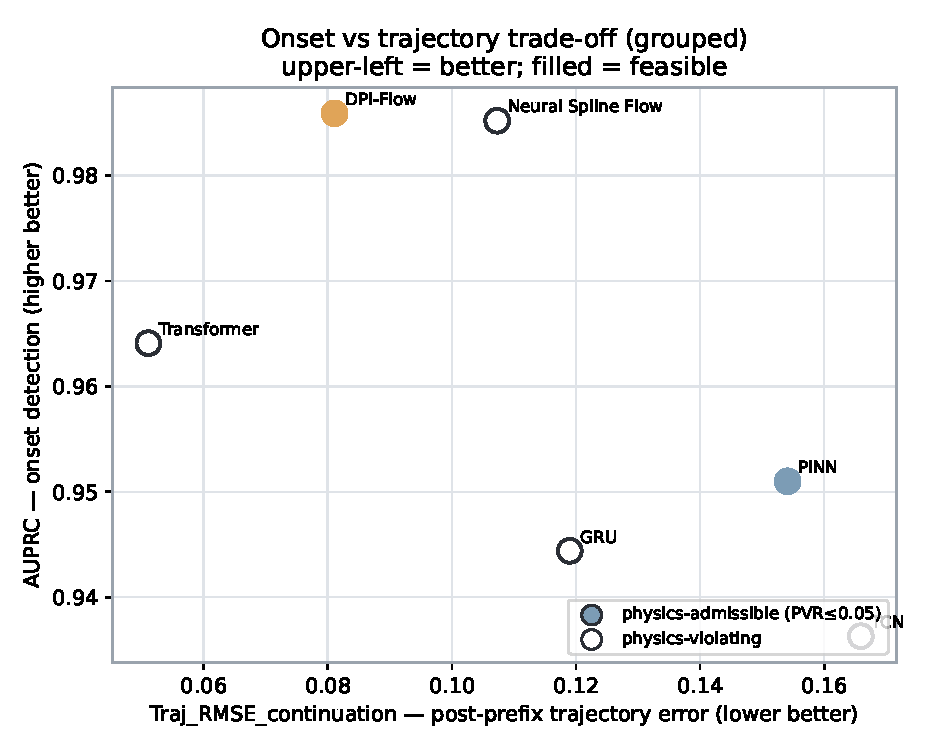
\includegraphics[width=\columnwidth]{Figures/fig_pareto.pdf}
\caption{Onset (AUPRC) vs.\ post-prefix trajectory error. Upper-left is better; filled markers are
physically admissible (PVR$\le 0.01$). Unconstrained baselines win a single axis but are infeasible or
omit structured outputs; DPI-Flow occupies the admissible frontier.}
\label{fig:pareto}
\end{figure}

\begin{figure}[t]
\centering
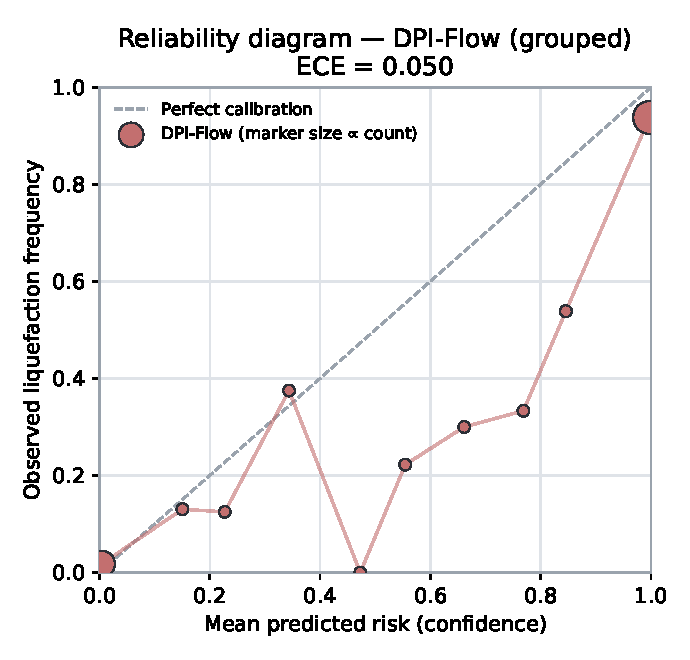
\includegraphics[width=\columnwidth]{Figures/fig_reliability.pdf}
\caption{Reliability diagram of onset risk for DPI-Flow under object-held-out CV; marker size encodes bin
count. Expected calibration error $0.050$.}
\label{fig:reliability}
\end{figure}

\section{Ablations and Robustness}
We ablate each component on the same object-held-out protocol (Figure~\ref{fig:ablation}).

\paragraph{The prefix is the dominant driver.} Removing the observed prefix (no-prefix stress test)
degrades onset AUPRC $0.970\!\to\!0.865$, post-prefix RMSE $0.080\!\to\!0.153$, worst-state
$0.146\!\to\!0.202$ and calibration ECE $0.080\!\to\!0.164$. Because the prefix is strictly pre-onset,
this confirms the prefix-conditioned formulation does real work and the onset signal is not a leakage
artifact.

\paragraph{Physical structure buys feasibility and event-time, at a trajectory cost.} Replacing the
analytical layer with a black-box decoder (\emph{wo-ode}) lowers raw post-prefix RMSE to $0.044$ but
\emph{worsens} $N_{\mathrm{liq}}$ log-MAE $0.328\!\to\!0.614$; removing both the layer and the monotone
projection (\emph{blackbox-raw}) drops physics violations from $\sim$0 to $0.225$. Thus the gain of the
structured model is not reducible to a cumulative-maximum post-processing: the ODE layer trades a little
raw trajectory accuracy for substantially better event-time prediction, feasibility, and the CRR/parameter
outputs.

\paragraph{Each remaining component contributes as designed.} Removing the monotone projection raises PVR
$0.004\!\to\!0.087$; removing conformal calibration drops coverage $0.849\!\to\!0.790$; replacing the
conditional flow with a plain Gaussian posterior worsens trajectory ($0.080\!\to\!0.087$, worst-state
$0.146\!\to\!0.152$). The model is robust to feature ablations: zeroing the Vs or grain-size features
changes all metrics by less than $0.02$.

\begin{figure}[t]
\centering
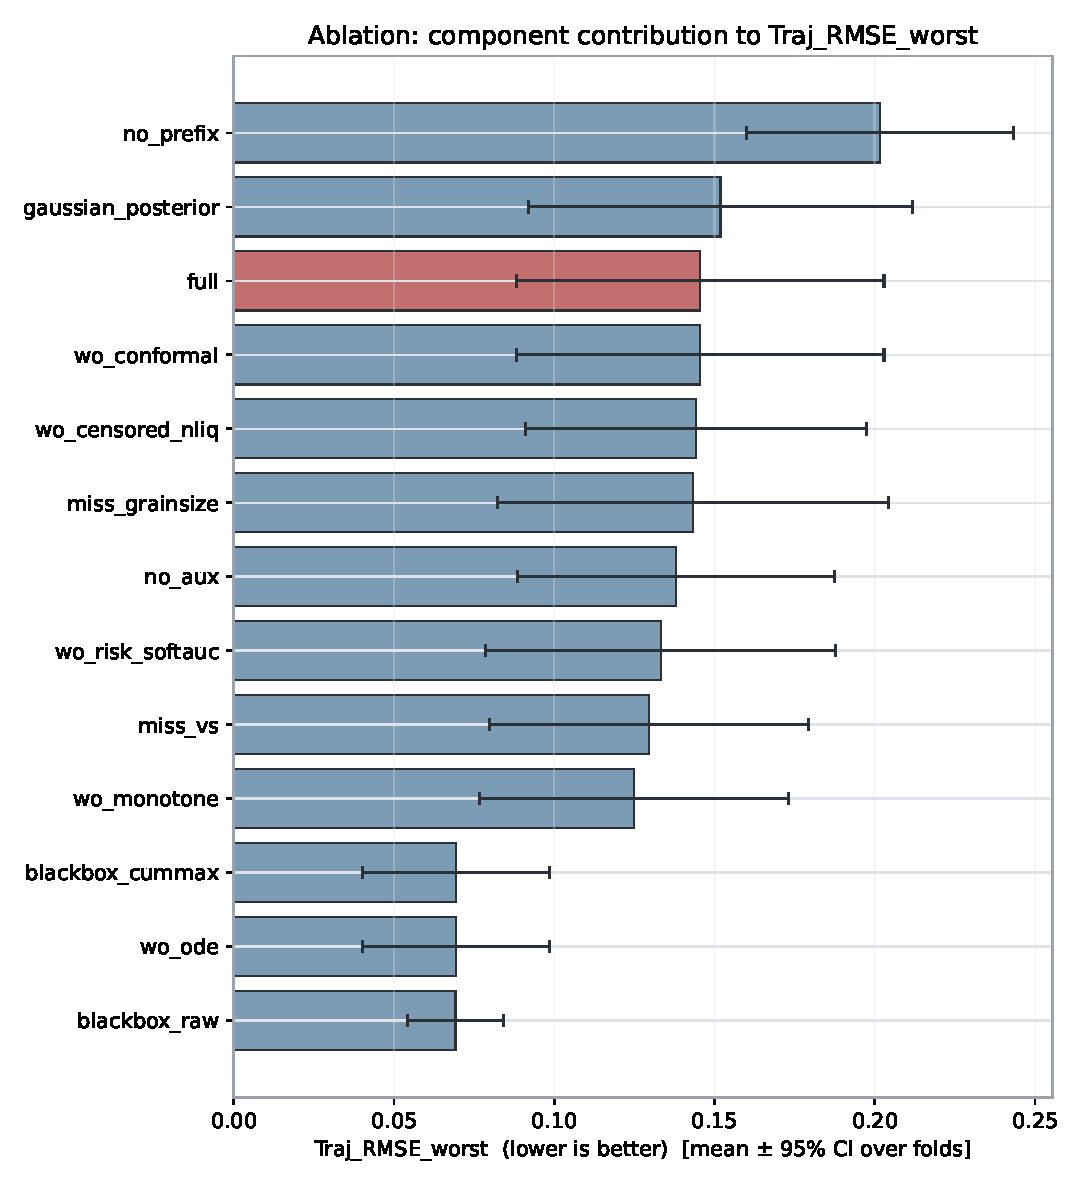
\includegraphics[width=\columnwidth]{Figures/fig_ablation.pdf}
\caption{Component contribution to worst-state post-prefix RMSE (mean $\pm$ 95\% CI over folds). ``full''
in accent; removing the prefix is by far the largest effect.}
\label{fig:ablation}
\end{figure}

\begin{figure}[t]
\centering
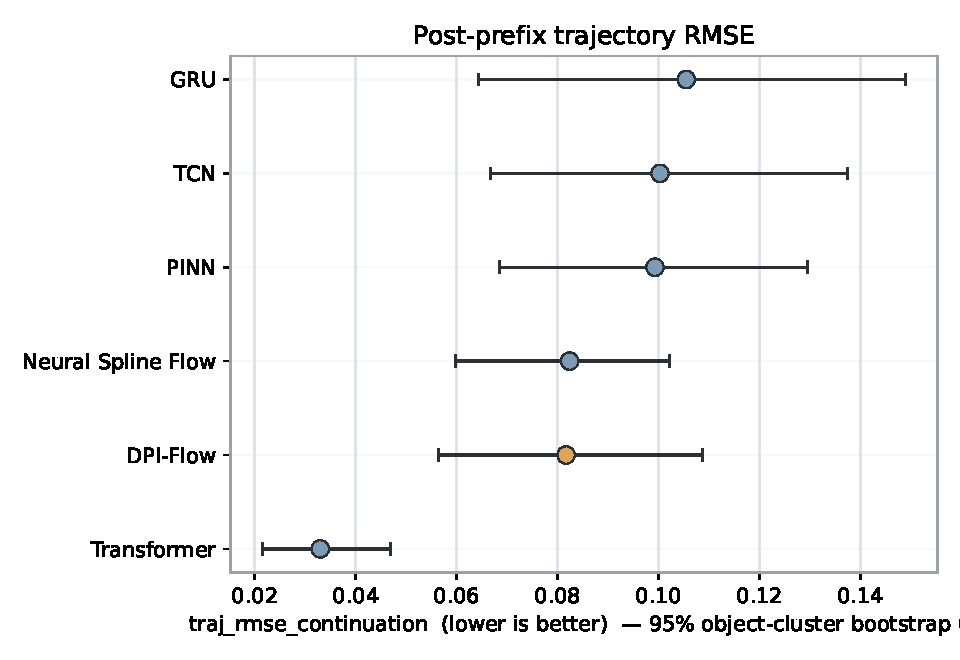
\includegraphics[width=\columnwidth]{Figures/fig_forest_traj.pdf}
\caption{Post-prefix trajectory RMSE across models with object-cluster bootstrap 95\% intervals (lower is
better). The Transformer leads raw trajectory but is physically infeasible (Table~\ref{tab:main}).}
\label{fig:forest}
\end{figure}

\section{Limitations}
CRR recovery is evaluated on a small number of measured-CRR sites per held-out fold; we therefore frame it
as \emph{exploratory recovery of measured CRR boundaries}, not robust cross-site generalization. The
monotone projection encodes an undrained accumulation assumption, not a universal physical law; zero
physics-violation rate is feasibility by construction, which we complement with black-box controls rather
than treat as empirical proof. The prefix-conditioned setting makes onset easier; we address this with
no-prefix and feature-ablation stress tests. The benchmark is a single laboratory campaign; lab-to-field
transfer is not claimed.

\section{Conclusion}
We presented DPI-Flow, a physics-constrained conditional flow for prefix-conditioned liquefaction
forecasting, and an object-held-out benchmark with honest, site-aware statistics. The defensible result is
not that one model wins everywhere, but that DPI-Flow provides the best \emph{physically admissible} Pareto
balance of onset accuracy, post-prefix trajectory quality, calibrated and flow-propagated uncertainty, and
structural feasibility, while uniquely recovering interpretable physical parameters and a CRR curve.
Scalar-only models (CatBoost) and unconstrained sequence models (Transformer) remain valuable points on
the frontier. A natural extension, \emph{DPI-SSM}, keeps the conditional-flow parameter-inference
front-end but replaces the fixed-form Euler integrator with a learned state-space recurrence as the
dynamics engine, trading some interpretability for trajectory capacity; we leave this, together with
onset-coherence diagnostics ($\mathrm{CRR}(N_{\mathrm{liq}})\!\approx\!\mathrm{CSR}$) and lab-to-field
transfer, to future work. We hope the released benchmark and ablation protocol make follow-up work in this
scarce, high-stakes regime easier to evaluate.

\bibliography{aaai2027}

\end{document}
